\documentclass[tikz,border=5pt]{standalone}
\begin{document}
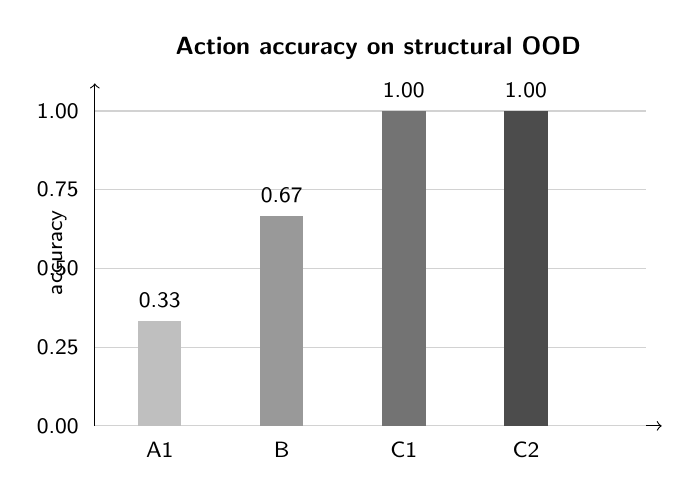
\begin{tikzpicture}[font=\sffamily\footnotesize]
\node[font=\sffamily\small\bfseries] at (3.6,4.8) {Action accuracy on structural OOD};
\draw[->] (0,0) -- (7.2,0);
\draw[->] (0,0) -- (0,4.35);
\node[rotate=90] at (-0.45,2.2) {accuracy};
\draw[gray!35] (0,0.000) -- (7.0,0.000);
\node[anchor=east] at (-0.08,0.000) {0.00};
\draw[gray!35] (0,1.000) -- (7.0,1.000);
\node[anchor=east] at (-0.08,1.000) {0.25};
\draw[gray!35] (0,2.000) -- (7.0,2.000);
\node[anchor=east] at (-0.08,2.000) {0.50};
\draw[gray!35] (0,3.000) -- (7.0,3.000);
\node[anchor=east] at (-0.08,3.000) {0.75};
\draw[gray!35] (0,4.000) -- (7.0,4.000);
\node[anchor=east] at (-0.08,4.000) {1.00};
\fill[black!25] (0.550,0) rectangle (1.100,1.333);
\node[anchor=north] at (0.825,-0.08) {A1};
\node[anchor=south] at (0.825,1.383) {0.33};
\fill[black!40] (2.100,0) rectangle (2.650,2.667);
\node[anchor=north] at (2.375,-0.08) {B};
\node[anchor=south] at (2.375,2.717) {0.67};
\fill[black!55] (3.650,0) rectangle (4.200,4.000);
\node[anchor=north] at (3.925,-0.08) {C1};
\node[anchor=south] at (3.925,4.050) {1.00};
\fill[black!70] (5.200,0) rectangle (5.750,4.000);
\node[anchor=north] at (5.475,-0.08) {C2};
\node[anchor=south] at (5.475,4.050) {1.00};
\end{tikzpicture}
\end{document}
